%!TEX root = thesis.tex
\section{Source Code}

	\begin{tabularx}{\textwidth}{@{}lX@{}}
		\toprule

		\textbf{Streaming WPS}
		& Extension for the 52°North WPS to allow of Inputs and Outputs over WebSockets.\\
		& \url{https://github.com/autermann/streaming-wps} \\
		\cmidrule(r){1-1}
		\cmidrule(l){2-2}

		\textbf{Matlab WPS}
		& Extension for the 52°North WPS to offer Matlab functions and scripts as OGC Web Processing Service algorithms.\\
		& \url{https://github.com/autermann/matlab-wps}\\
		\cmidrule(r){1-1}
		\cmidrule(l){2-2}

		\textbf{streaming-wps-js}
		& Streaming WPS JavaScript Bindings\\
		& \url{https://github.com/autermann/streaming-wps-js}\\
		\cmidrule(r){1-1}
		\cmidrule(l){2-2}

		\textbf{WPS Commons}
		& 52°North WPS convenience classes and bootstrapping code.\\
		& \url{https://github.com/autermann/wps-commons}\\
		\cmidrule(r){1-1}
		\cmidrule(l){2-2}

		\textbf{Matlab Connector}
		& Matlab function execution on (pooled) remote Matlab instances.\\
		& \url{https://github.com/autermann/matlab-connector}\\
		\cmidrule(r){1-1}
		\cmidrule(l){2-2}

		\textbf{Lake-Analyzer}
		& Matlab source code for Lake Analyzer\\
		& \url{https://github.com/autermann/Lake-Analyzer}\\
		\cmidrule(r){1-1}
		\cmidrule(l){2-2}

		\textbf{YAML API}
		& A Jackson-like API to read and create YAML nodes (based on SnakeYAML).\\
		& \url{https://github.com/autermann/yaml}\\
		\bottomrule
	\end{tabularx}

\section{Figures}
	\begin{figure}[!htb]
		\centering
		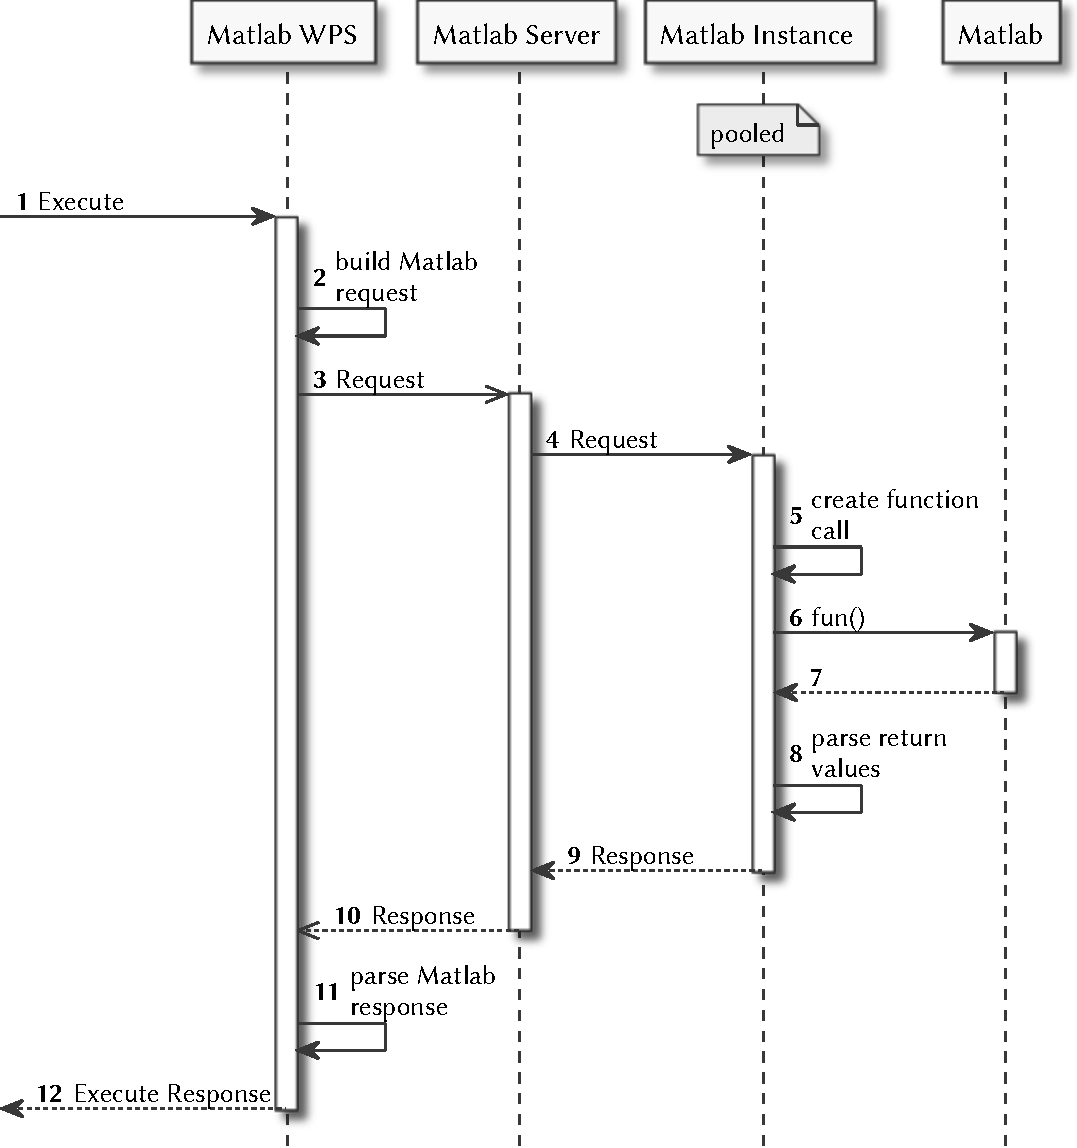
\includegraphics[width=.8\textwidth]{figures/sequence-diagramm-mwps.pdf}
		\caption{\label{fig:sd:mwps} Sequence diagram of the Matlab WPS.} %182x194
	\end{figure}
	\begin{figure}[!htb]
		\centering
		% !TEX root = ../thesis.tex
\begin{tikzpicture}
	\scriptsize
	\tikzset{
	  ibox/.style = {draw, fill=string!50,  minimum width=4cm, minimum height=.6cm},
	  pbox/.style = {draw, fill=comment!50, minimum width=4cm, minimum height=.6cm},
	  obox/.style = {draw, fill=keyword!50, minimum width=4cm, minimum height=.6cm},
	  every node/.style={font=\sffamily},
	}
	\draw[>->] (-2.4,3.6) -- (11.4,3.6);
	%\draw[]   (-2.4,3.6) -- (-2.4, -6);
	\draw[>->] (-2.4, -6) -- (11.4, -6);

	\draw[dotted] (-2.0,-6) -- (-2.0,3.6);
	\draw[dotted] (-1.0,-6) -- (-1.0,3.6);
	\draw[dotted] (-0.0,-6) -- (-0.0,3.6);
	\draw[dotted] (1.0,-6) -- (1.0,3.6);
	\draw[dotted] (2.0,-6) -- (2.0,3.6);
	\draw[dotted] (3.0,-6) -- (3.0,3.6);
	\draw[dotted] (4.0,-6) -- (4.0,3.6);
	\draw[dotted] (5.0,-6) -- (5.0,3.6);
	\draw[dotted] (6.0,-6) -- (6.0,3.6);
	\draw[dotted] (7.0,-6) -- (7.0,3.6);
	\draw[dotted] (8.0,-6) -- (8.0,3.6);
	\draw[dotted] (9.0,-6) -- (9.0,3.6);
	\draw[dotted] (10.0,-6) -- (10.0,3.6);
	\draw[dotted] (11.0,3.6) -- (11.0,-6) node [below] {Time};

	\node [xshift=-1.5cm,yshift=2.4cm] {(a)};
	\node [ibox,yshift=3.0cm,xshift=1cm] (input1) {Input Upload};
	\node [pbox,yshift=2.4cm,xshift=5cm] (processing1) {Processing};
	\node [obox,yshift=1.8cm,xshift=9cm] (output1) {Output Download};

	\draw[dashed] (-2.4, 1.2) -- (11.4, 1.2);

	\node [xshift=-1.5cm,yshift=0cm] {(b)};
	\node [ibox,yshift= .6cm,xshift=1cm] (input2) {Input Stream};
	\node [pbox,yshift= .0cm,xshift=2cm] (processing2) {Processing};
	\node [obox,yshift=-.6cm,xshift=6cm] (output2) {Output Stream};

	\draw[dashed] (-2.4, -1.2) -- (11.4, -1.2);

	\node [xshift=-1.5cm,yshift=-2.4cm] {(c)};
	\node [ibox,yshift=-1.8cm,xshift=1cm] (input3) {Input Stream};
	\node [pbox,yshift=-2.4cm,xshift=5cm] (processing3) {Processing};
	\node [obox,yshift=-3.0cm,xshift=6cm] (output3) {Output Stream};

	\draw[dashed] (-2.4, -3.6) -- (11.4, -3.6);

	\node [xshift=-1.5cm,yshift=-4.8cm] {(d)};
	\node [ibox,yshift=-4.2cm,xshift=1cm] (input4) {Input Stream};
	\node [pbox,yshift=-4.8cm,xshift=2cm] (processing4) {Processing};
	\node [obox,yshift=-5.4cm,xshift=3cm] (output4) {Output Stream};
\end{tikzpicture}
		\caption{\label{fig:streaming}Four different types of processing data: (a) conventional processing, (b) streaming input data (c) streaming output data, (d) full input and output streaming \citep[based on][]{foerster2012live}.}
	\end{figure}
	\begin{figure}[!htb]
		\centering
		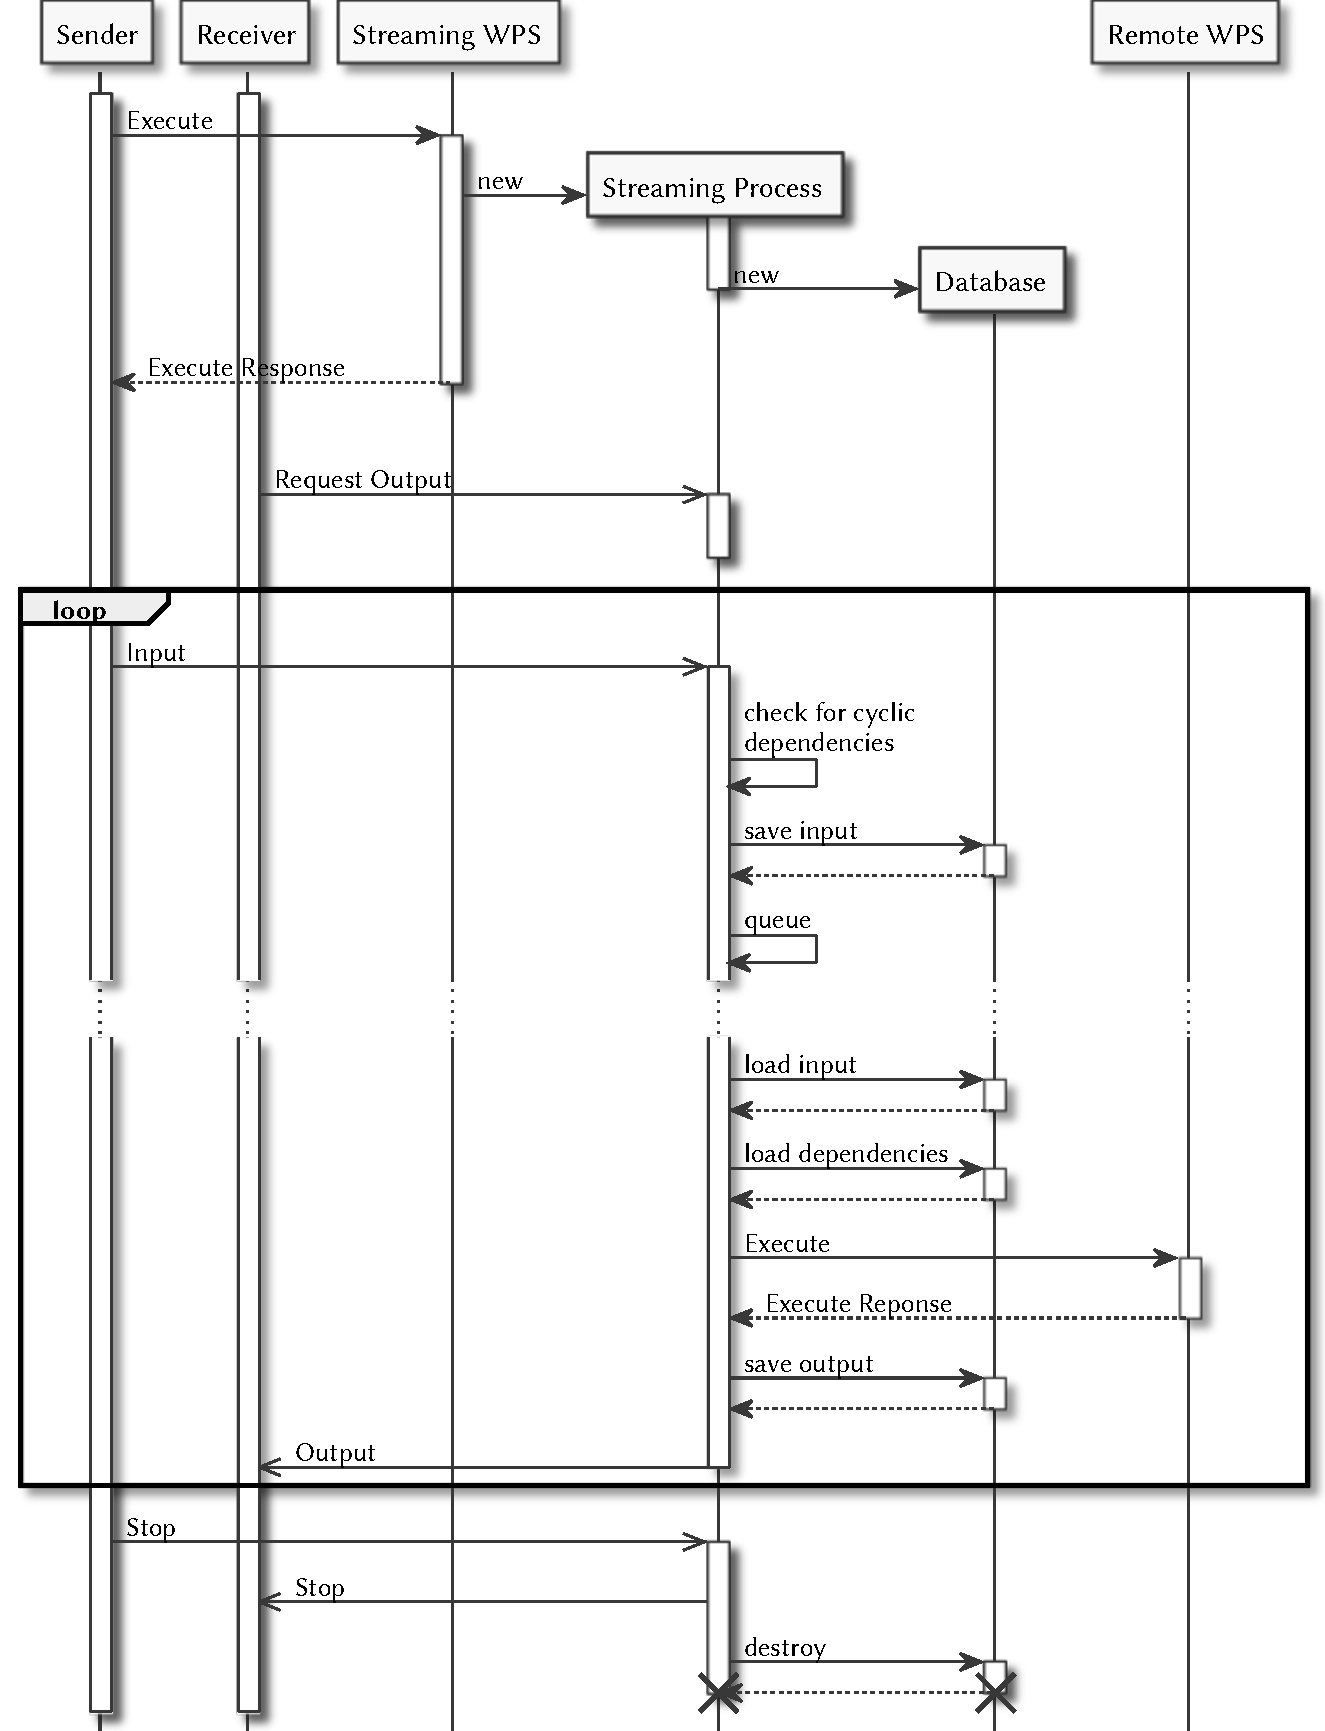
\includegraphics[width=.7868\textwidth]{figures/sequence-diagramm-swps.pdf} % 179x274
		\caption{\label{fig:sd:swps} Sequence diagram of the Streaming WPS.}
	\end{figure}
	\begin{figure}[!htb]
		\centering
		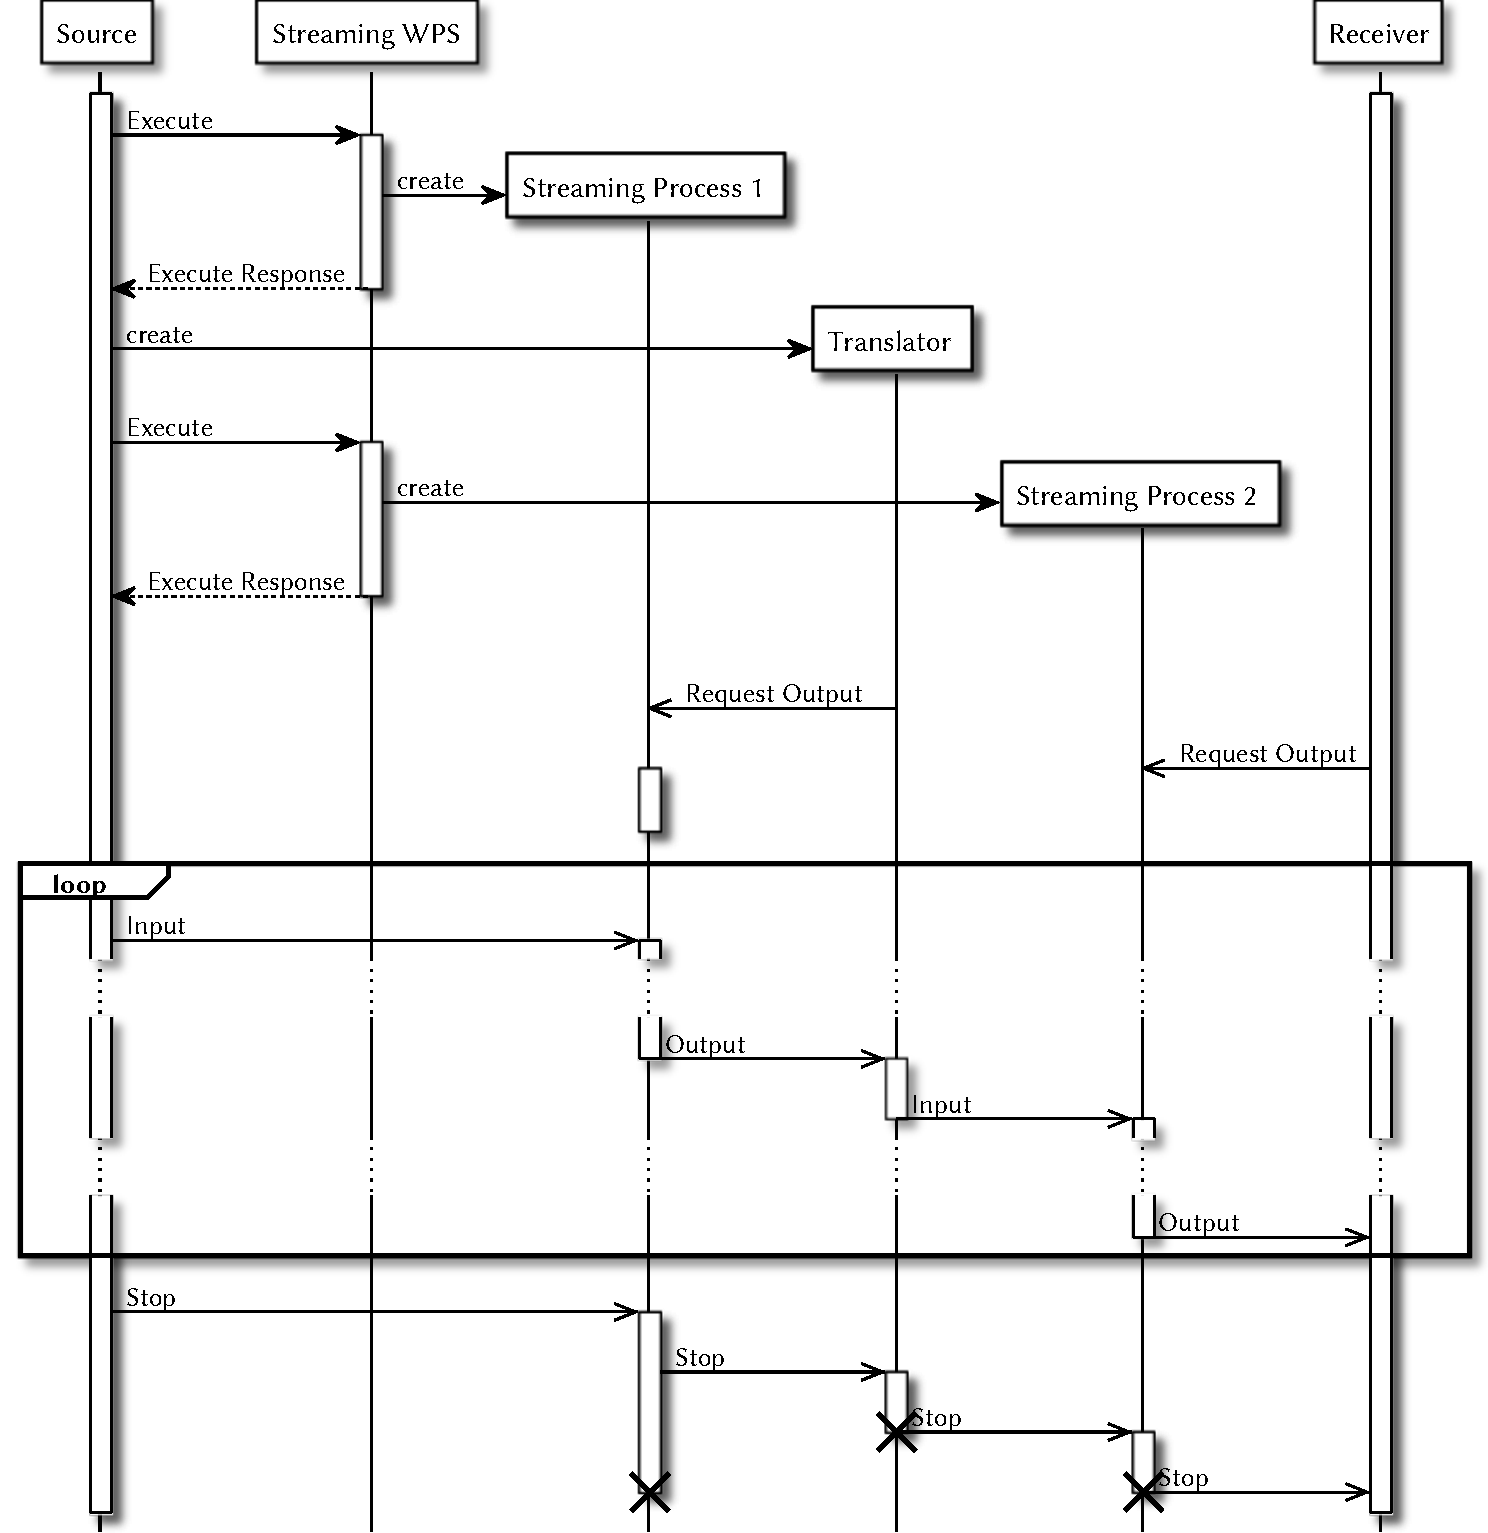
\includegraphics[width=\textwidth]{figures/sequence-diagramm-chain.pdf} % 179x274
		\caption{\label{fig:sd:chain} Sequence diagram of chaining two different streaming processes.}
	\end{figure}
	\begin{figure}[!htb]
		\centering
		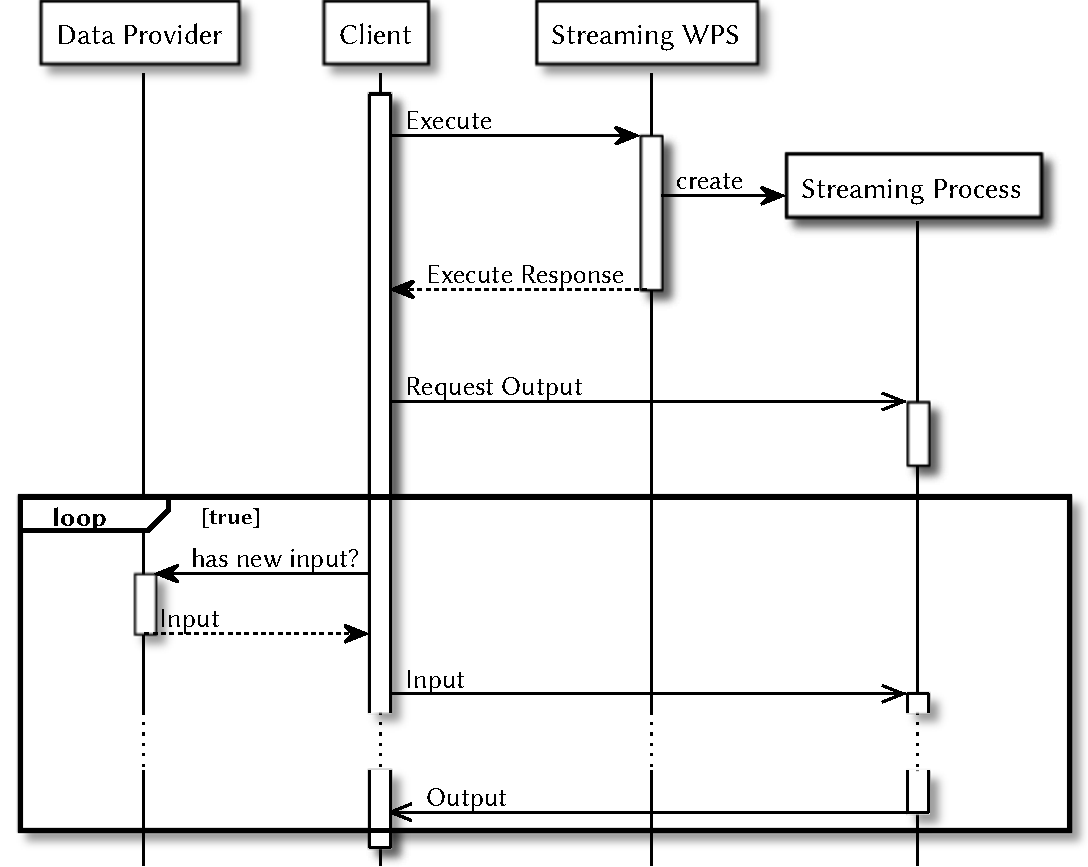
\includegraphics[width=.7868\textwidth]{figures/sequence-diagramm-polling.pdf}
		% 179x274
		\caption{\label{fig:sd:polling} Sequence diagram of polling inputs of the Streaming WPS.}
	\end{figure}
	\begin{figure}[!htb]
		\centering
		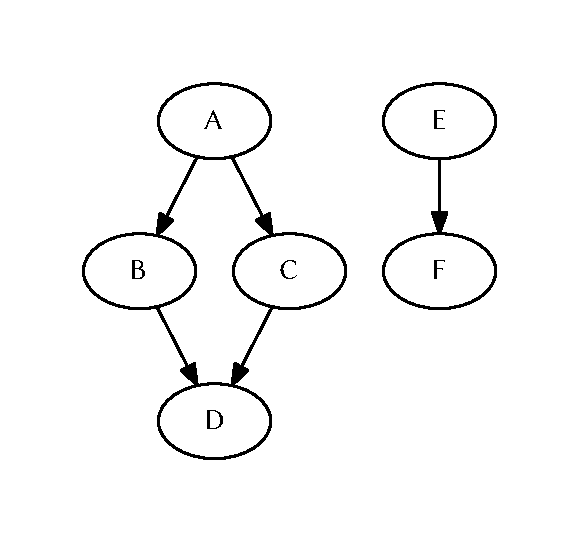
\includegraphics[width=.4474\textwidth]{figures/unordered-graph.pdf} % 98x92
		\caption{\label{fig:graph:unordered} Example for a dependency graph consisting of two independent subgraphs.}
	\end{figure}
	\begin{figure}[!htb]
		\centering
		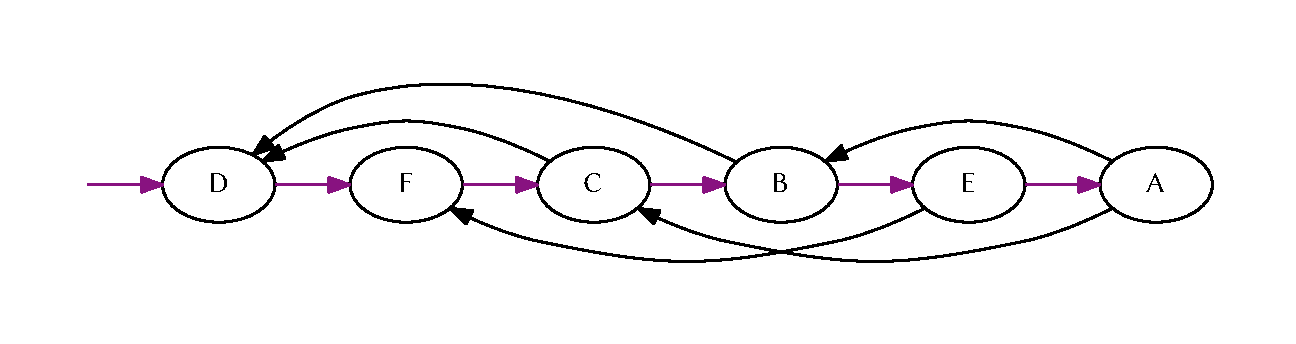
\includegraphics[width=1\textwidth]{figures/ordered-graph.pdf} % 219x58
		\caption{\label{fig:graph:ordered} Possible execution/topological order of the dependency graph in Figure \ref{fig:graph:unordered}. Black arrows represent dependence to another vertex, colored arrows the execution order.}
	\end{figure}

\section{Listings}
	\includecode[Matlab]{matlab-add-function.m}{\label{lst:matlab:example:fun}Matlab example function that represents a simple addition.}
	\includecode[YAML,morekeywords={function,connection,identifier,version,inputs,outputs,type}]{matlab-add-process-configuration.yaml}{\label{lst:matlab:example:yaml}Matlab process configuration describing the function in Listing \ref{lst:matlab:example:fun}.}
	\includecode[XML]{matlab-add-process-description.xml}{\label{lst:matlab:example:desc}Process description generated from the configuration in Listing \ref{lst:matlab:example:yaml}.}
	\includecode[XML]{streaming-input-streaming.xml}{\label{lst:streaming:input:streaming}Example for a Streaming WPS streaming inputs.}
	\includecode[XML]{streaming-input-static.xml}{\label{lst:streaming:input:static}Example for a Streaming WPS static inputs.}
	\includecode[XML]{streaming-input-reference.xml}{\label{lst:streaming:input:reference}Example for a Streaming WPS reference input.}
	\includecode[XML]{streaming-message-input.xml}{\label{lst:streaming:message:input}Example for a Streaming WPS input message.}
	\includecode[XML]{streaming-message-output.xml}{\label{lst:streaming:message:output}Example for a Streaming WPS output message.}
	\includecode[XML]{streaming-message-output-request.xml}{\label{lst:streaming:message:output-request}Example for a Streaming WPS output request message.}
	\includecode[XML]{streaming-message-error.xml}{\label{lst:streaming:message:error}Example for a Streaming WPS error message.}
	\includecode[XML]{streaming-message-describe.xml}{\label{lst:streaming:message:describe}Example for a Streaming WPS describe message.}
	\includecode[XML]{streaming-message-description.xml}{\label{lst:streaming:message:description}Example for a Streaming WPS description message.}
	\includecode[XML]{streaming-message-stop.xml}{\label{lst:streaming:message:stop}Example for a Streaming WPS stop message.}

\section{Tables}
	\begin{table}[!htb]
		\sffamily\centering
		\caption{\label{tab:matlab:typemapping}Type Mapping between Matlab and WPS Data}
		\begin{tabular}{@{}llcc@{}}
			\toprule
			&
			& \multicolumn{2}{b}{Matlab Type}\\
			\cmidrule(l){3-4}
			\multicolumn{1}{@{}b}{}
			& \multicolumn{1}{b}{Data}
			& \multicolumn{1}{b}{For single inputs}
			& \multicolumn{1}{b@{}}{For multiple inputs}\\
			\cmidrule(rl){2-2}
			\cmidrule(rl){3-3}
			\cmidrule(l){4-4}
			\textbf{Complex}      & \textit{any} & String  & Cell \\\midrule
			\textbf{Bounding Box} & -            & -       & -    \\\midrule
			\textbf{Literal}      & xs:int       & Numeric & Array\\
							      & xs:boolean   & Numeric & Array\\
							      & xs:dateTime  & Numeric & Array\\
							      & xs:double    & Numeric & Array\\
							      & xs:float     & Numeric & Array\\
							      & xs:byte      & Numeric & Array\\
							      & xs:short     & Numeric & Array\\
							      & xs:int       & Numeric & Array\\
							      & xs:long      & Numeric & Array\\
							      & xs:string    & String  & Cell \\
							      & xs:anyURI    & String  & Cell \\
			\bottomrule
		\end{tabular}
	\end{table}